\chapter{案例實驗}
\section{實驗環境與參數}
此次實驗採用 FEMU 作為 SSD 模擬器,FEMU 是一個由 QEMU \cite{bellard2005qemu}修改而成的模擬器\cite{210518},支援模擬下列幾種 SSD
\begin{itemize}
    \item NoSSD
    \item Black-box SSD
    \item Open-Channel SSD
    \item Zoned-Namespace (ZNS) SSD
\end{itemize}
實驗環境參數如同下列所述:
\begin{itemize}
    \item Linux Kernel 5.10.83
    \item 4 核心
    \item 5G 記憶體
    \item 模擬 4G 硬碟
\end{itemize}

\section{實驗規劃}
\indent
本論文將以在 Linux 上常用的硬碟效能檢測工具 FIO (Flexible I/O tester) 來實測效能差異。實驗將分為兩個部分,第一部分是測試在同樣的資料量底下,採用原版的 LightNVM 與我們修改過的 LightNVM 所產生的 Garbage Collection 次數差異,第二部分為在同樣時間下,採用原版的 LightNVM 與我們修改過的 LightNVM 所寫入的資料量差異。以這兩種實驗來確認採用本論文的設計實作是否對於 Garbage Collection 效率有所幫助。

\section{實驗一:Garbage Collection 次數比較}\label{s4.2}

\indent
表\ref{t4.1}跟圖\ref{f4.1}為在同樣資料量情況下,使用原版以及修改過後的 LightNVM 進行Garbage Collection 次數之比較,從表中可見隨著資料量增加,兩邊所產生的 Garbage Colleciton 次數也隨之增加,而我們所修改的 LightNVM 版本產生的次數與原版 LightNVM 比較起來,減少的比例由 4G 到 64G 依序為 44\%、61\%、65\%、66\%、68\%,平均大約減少了60.8\%;稍微要注意的是,由於 LightNVM 本身架構,這邊的次數代表的是有多少 Line 被 Garbage Collection 處理過。

\begin{table}[H]
    \begin{center}
        \caption{在同樣資料量情況下,Garbage Collection 次數比較}\label{t4.1}
        \begin{tabular}{|c|c|c|}\hline
                & 使用原版 LightNVM 的 GC 次數 & 使用修改版 LightNVM 的 GC次數 \\\hline
            4G  & 25                    & 14                    \\\hline
            8G  & 159                   & 62                    \\\hline
            16G & 482                   & 170                   \\\hline
            32G & 1144                  & 392                   \\\hline
            64G & 2493                  & 812                   \\\hline
        \end{tabular}
    \end{center}
\end{table}

\begin{figure}[H]
    \centering
    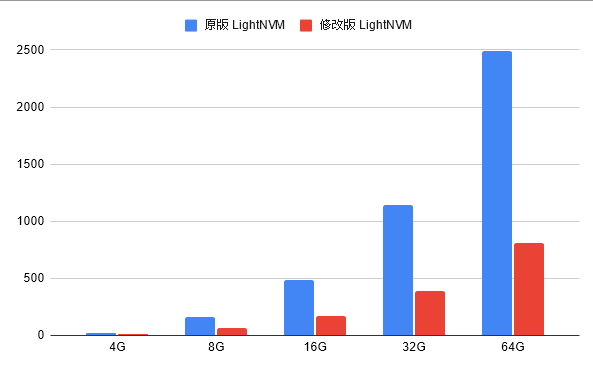
\includegraphics[width=0.8\textwidth]{picture/ch4/gc_chart.png}
    \caption{Garbage Collection 次數比較圖 (單位:次數)}
    \label{f4.1}
\end{figure}

\section{實驗二:寫入資料量比較}\label{s4.3}

\indent
表\ref{t4.2}跟圖\ref{f4.2}為在同樣時間情況下,使用原版以及修改過後的 LightNVM 進行資料寫入量之比較,從表中可見隨著時間增加,兩邊所產生的寫入資料量也隨之增加,而我們所修改的 LightNVM 版本產生的次數與原版 LightNVM 比較起來,增加的比例由 1 分鐘 到 4 分鐘 依序為 10.3\%、4.8\%、1.6\%、5.1\%,平均大約增加了 5.45\%。

\begin{table}[H]
    \begin{center}
        \caption{在同樣時間情況下,寫入資料量比較}\label{t4.2}
        \begin{tabular}{|c|c|c|}\hline
                & 使用原版 LightNVM 的 寫入資料量 & 使用修改版 LightNVM 的寫入資料量 \\\hline
            1分鐘 & 193GiB                & 213GiB                \\\hline
            2分鐘 & 431GiB                & 452GiB                \\\hline
            3分鐘 & 669GiB                & 680GiB                \\\hline
            4分鐘 & 862GiB                & 906GiB                \\\hline
        \end{tabular}
    \end{center}
\end{table}

\begin{figure}[H]
    \centering
    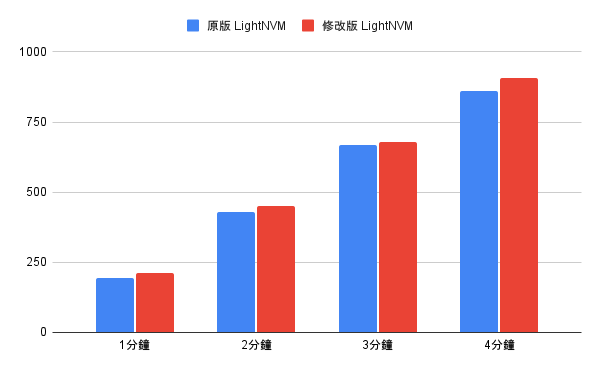
\includegraphics[width=0.8\textwidth]{picture/ch4/write_chart.png}
    \caption{寫入資料量比較圖 (單位:GiB)}
    \label{f4.2}
\end{figure}